\documentclass[dvipsnames,beamer,10pt]{standalone}

\usepackage{textcomp}
\usepackage{lmodern}

\usepackage{tikz}
\usepackage{arrayjob}




\usetikzlibrary{positioning,decorations.pathreplacing,fit}
\usetikzlibrary{decorations.markings,arrows.meta,shapes.arrows,arrows}
\usetikzlibrary{bending}
\usetikzlibrary{calc}

\definecolor{mygreen}{RGB}{0,128,80}
\colorlet{darkgreen}{mygreen!90!black}

\providecommand{\adlog}{\textcolor{red}{a}}
\providecommand{\bdlog}{\textcolor{blue}{b}}
\providecommand{\cdlog}{\textcolor{Plum}{c}}
\providecommand{\ddlog}{\textcolor{OliveGreen}{d}}
\providecommand{\dlog}[2]{\textcolor{#1}{#2}}
\providecommand{\ua}[1]{\dlog{red}{#1}}
\providecommand{\ub}[1]{\dlog{blue}{#1}}
\providecommand{\uc}[1]{\dlog{Plum}{#1}}
\providecommand{\ud}[1]{\dlog{OliveGreen}{#1}}



%\DeclareMathSizes{10.0}{12}{5}{4}


\begin{document}




\begin{standaloneframe}

\resizebox{1\textwidth}{!}{



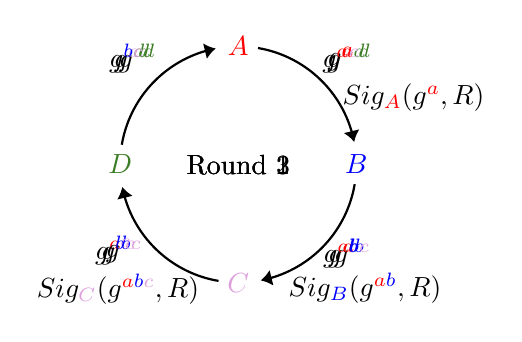
\begin{tikzpicture}[
		mycircle/.style= {
		fill,circle, inner sep=1pt
		},
		>={Latex[length=4pt,width=6pt]},<->,shorten <= 1pt,
		main node/.style={},
		every path/.style={
		        thick
		    }
	]
		

	\newcommand*{\MainNum}{4}
	  \newcommand*{\MainRadius}{1.5cm} 
	  \newcommand*{\MainStartAngle}{180}
	
	  % Print main nodes, node names: p1, p2, ...
		\coordinate (M) at (0,0);

		 
		\node (u1) at ({-1*360/\MainNum + \MainStartAngle}:\MainRadius) {\ua{$A$}};
		\node[inner sep=1pt] (m_1) at ({-1*360/\MainNum + 135}:\MainRadius + 0.4cm) {};
		
		\node (u2) at ({-2*360/\MainNum + \MainStartAngle}:\MainRadius) {\ub{$B$}};
		\node[inner sep=1pt] (m_2) at ({-2*360/\MainNum + 135}:\MainRadius + 0.4cm) {};
		
		\node (u3) at ({-3*360/\MainNum + \MainStartAngle}:\MainRadius) {\textcolor{Plum}{$C$}};
		\node[inner sep=1pt] (m_3) at ({-3*360/\MainNum + 135}:\MainRadius + 0.4cm) {};
		
		\node (u4) at ({-4*360/\MainNum + \MainStartAngle}:\MainRadius) {\textcolor{OliveGreen}{$D$}};
		\node[inner sep=1pt] (m_4) at ({-4*360/\MainNum + 135}:\MainRadius + 0.4cm) {};
		 
		 
		 

	
	  % Calculate the angle between the equal sides of the triangle
	  % with side length \MainRadius, \MainRadius and radius of circle node
	  % Result is stored in \p1-angle, \p2-angle, ...
	  \foreach \i in {1, ..., \MainNum} {
	    \pgfextracty{\dimen0 }{\pgfpointanchor{u\i}{north}} 
	    \pgfextracty{\dimen2 }{\pgfpointanchor{u\i}{center}}
	    \dimen0=\dimexpr\dimen2 - \dimen0\relax 
	    \ifdim\dimen0<0pt \dimen0 = -\dimen0 \fi
	    \pgfmathparse{2*asin(\the\dimen0/\MainRadius/2)}
	    \global\expandafter\let\csname p\i-angle\endcsname\pgfmathresult
	  }
	
	  % Draw the arrow arcs
	  \foreach \i [evaluate=\i as \nexti using {int(mod(\i, \MainNum)+1}]
	  in {1, ..., \MainNum} {  
	    \pgfmathsetmacro\StartAngle{   
	      (\i-1)*360/\MainNum + \MainStartAngle
	      + \csname p\i-angle\endcsname
	    }
	    \pgfmathsetmacro\EndAngle{
	      (\nexti-1)*360/\MainNum + \MainStartAngle
	      - \csname p\nexti-angle\endcsname
	    }
	    \ifdim\EndAngle pt < \StartAngle pt
	      \pgfmathsetmacro\EndAngle{\EndAngle + 360}
	    \fi
	    \draw[<-]
	      (M) ++(\StartAngle:\MainRadius)
	      arc[start angle=\StartAngle, end angle=\EndAngle, radius=\MainRadius]
	    ;
	  }
	

%	\uncover<+>{
%		\node[above=-2pt of u1] {$g^{\adlog}$};
%		\node[right=-4pt of u2] {$g^{\bdlog}$};
%		\node[below=-2pt of u3] {$g^{\cdlog}$};
%		\node[left=-4pt of u4] {$g^{\ddlog}$};
%	}
	
	\pause
	
	\uncover<+,+(3),+(6)>{
		\node at (M) {Round 1};
		\node[xshift=-1pt] (ga)  at (m_1) {$g^{\adlog}$};
	}


	\uncover<+,+(3),+(6)>{
		\node at (M) {Round 2};
		\node[xshift=1pt,yshift=6pt] (gb) at (m_2) {$g^{\adlog\bdlog}$};
	}
	
	\uncover<+,+(3),+(6)>{
		\node at (M) {Round 3};
		\node[xshift=-5pt,yshift=7pt] (gc)  at (m_3) {$g^{\adlog\bdlog\cdlog}$};
	}
	
	\uncover<+>{
		\node[xshift=1pt,yshift=6pt] at (m_2) {$g^{\bdlog}$};
		\node[xshift=-5pt,yshift=7pt] at (m_3) {$g^{\cdlog}$};
		\node[]  at (m_4) {$g^{\ddlog}$};	
	}
	
	\uncover<+>{
		\node[xshift=1pt] at (m_1) {$g^{\adlog\ddlog}$};
		\node[xshift=-5pt,yshift=7pt] at (m_3) {$g^{\bdlog\cdlog}$};
		\node[]  at (m_4) {$g^{\cdlog\ddlog}$};
	}
	
	\uncover<+>{
		\node[xshift=1pt] at (m_1) {$g^{\adlog\cdlog\ddlog}$};
		\node[xshift=1pt,yshift=6pt] at (m_2) {$g^{\adlog\bdlog\cdlog}$};
		\node[]  at (m_4) {$g^{\bdlog\cdlog\ddlog}$};
	}
	
	
	
	\uncover<+>{
		\node[below right = -0.1 and -12pt of ga] {$Sig_{\ua{A}}(g^{\adlog},R)$};
	}
	
	\uncover<+>{
		\node[below left = -0.2 and -1.7cm of gb] {$Sig_{\ub{B}}(g^{\adlog\bdlog},R)$};
	}
	
	\uncover<+>{
		\node[below right = -0.15 and -1.6cm of gc] {$Sig_{\uc{C}}(g^{\adlog\bdlog\cdlog},R)$};
	}



\end{tikzpicture}


}

\end{standaloneframe}


\end{document}